\documentclass[12pt]{iopart}

\expandafter\let\csname equation*\endcsname\relax
\expandafter\let\csname endequation*\endcsname\relax
\usepackage{amsmath}
\usepackage{amssymb}
\usepackage{graphicx}
\usepackage{booktabs}
\usepackage{longtable}
\usepackage{url}
\usepackage{bm}
\usepackage{array}
\usepackage{xcolor}

\newcommand{\mpl}{M_{\rm Pl}}
\newcommand{\LCDM}{\Lambda{\rm CDM}}
\newcommand{\dd}{\mathrm{d}}
\providecommand{\Tr}{\mathrm{Tr}}
\newcommand{\STr}{\mathrm{STr}}
\newcommand{\cO}{\mathcal O}
\newcommand{\cF}{\mathcal F}
\newcommand{\cT}{\mathcal T}
\newcommand{\cR}{\mathcal R}
\newcommand{\cL}{\mathcal L}
\newcommand{\cH}{\mathcal H}
\newcommand{\cK}{\mathcal K}
\newcommand{\cS}{\mathcal S}
\newcommand{\Q}{\mathcal Q}
\newcommand{\Y}{\mathcal Y}
\newcommand{\Om}{\Omega}
\newcommand{\provisional}{\textit{provisional}}

\begin{document}

\title{From an interacting ultraviolet fixed point to a reproducible cyclic cosmology:\\
a source-explicit Wilsonian construction and cross-machine validation}

\author{Panagiotis Karmiris}
\address{Independent Researcher, Greece}

\submitto{Classical and Quantum Gravity}

\begin{abstract}
We present a source-explicit construction that connects a non-perturbative functional-renormalization-group (FRG) fixed point to a low-energy cyclic cosmology through an explicit Wilsonian decoupling transition.  The ultraviolet (UV) calculation is performed in a retained functional space containing three one-dimensional functions, four two-dimensional functions, and seven finite couplings.  A massive vector alignment sector is then evolved together with the functional system until the dimensionless physical threshold variable $\mu_A=m_A^2/(Z_A k^2)$ reaches a prescribed matching value.  At that scale the heavy vector is integrated out, generating a controlled derivative expansion through the retained $p^8$ order.  The infrared (IR) theory contains three light propagating degrees of freedom, two tensor and one scalar, while the full microscopic constrained system contains six physical degrees of freedom before decoupling.

The source-exact merger is solved numerically in a 695-dimensional representation.  At the canonical $\mu_A=7$ handoff we find $t_{\rm match}=-3.97664237$, $k_{\rm match}=1.87484842\times10^{-2}\mpl$, a minimum tensor denominator of $0.645538$, and a maximum componentwise ordinary-differential-equation defect of $7.68\times10^{-7}$.  Dense off-grid projection tests give a maximum polynomial-projector residual of $9.84\times10^{-7}$.  The current matching bookkeeping distinguishes Wilson-coefficient displacements from post-matching errors: the largest reported retained coefficient displacement is $5.89\times10^{-4}$, whereas the reported unrepresented derivative remainder is $5.21\times10^{-5}$.  A strict raw-projector ledger with threshold $R_{\rm match}<10^{-4}$ is retained as a pre-submission reproducibility gate rather than assumed from these summary numbers.

Across the nonsingular bounce, scalar and tensor perturbations admit regular canonical variables and finite transfer matrices.  Independent recomputation reproduces a scalar transfer amplitude $0.93968314$, corresponding to $P_{\cal R}^{+}/P_{\cal R}^{-}=0.8830044$ on observable scales, with symplectic residual $5.2\times10^{-13}$ and Radau--DOP853 transfer disagreement $2.8\times10^{-11}$; the tensor transfer is consistent with the identity at the tested precision.  A modified CLASS implementation is then sampled with four production MCMC chains.  At the present manuscript-draft freeze those production chains are still running, so posterior-dependent headline values and posterior figures are not yet frozen.  A previously frozen validation snapshot was independently replayed and satisfied the declared convergence threshold, and its held-out ACT DR6 CMB lensing, twelve $f\sigma_8$ measurements, and eight $E_G$ measurements gave $\Delta\chi^2=+0.170$ relative to a matched $\LCDM$ comparator over the 30-point validation vector.  These validation-snapshot numbers are retained as methodological cross-checks and will be regenerated from the final production chains before submission.

The central purpose of this work is methodological as much as phenomenological: every major transition---fixed point, UV-to-IR flow, heavy-field decoupling, bounce transfer, Boltzmann implementation, chains, and held-out likelihoods---is associated with a machine-readable authority package and an independent numerical replay.  The results support an asymptotically safe Wilsonian UV-to-IR construction within the declared functional truncation; they do not constitute an all-orders proof of UV completeness.  We provide the derivations, numerical tolerances, provenance rules, failure modes, and falsifiability criteria needed for external groups to reproduce or refute the construction.
\end{abstract}

\maketitle

\section{Introduction}
\label{sec:intro}

The standard cosmological model succeeds on an extraordinary range of scales, but its dark sector remains largely phenomenological and its classical extrapolation to the highest curvatures is incomplete.  At the same time, modern observational cosmology increasingly permits theories of gravity to be tested through a joint chain extending from the covariant action to background evolution, linear perturbations, Boltzmann transfer functions, large-scale-structure observables, and lensing.  Relativistic scalar--vector models provide one route to modified phenomenology while preserving a covariant field-theory formulation \cite{SkordisZlosnik2021,SkordisZlosnik2022,BatakiSkordisZlosnik2024,RosaZlosnik2024}.  Type-II minimally modified gravity and its VCDM realization provide a complementary route in which the cosmological background can differ from general relativity without introducing the conventional additional scalar graviton \cite{DeFeliceMukohyamaPookkillath2021,DeFeliceMaedaMukohyamaPookkillath2022,GanzMartensMukohyamaNamba2023}.  These developments motivate asking whether a constrained gravitational model can be connected not merely to an IR fit, but to a non-perturbative UV construction and a controlled Wilsonian matching step.

The gravitational asymptotic-safety programme offers a concrete framework for this question.  The central hypothesis is that the UV limit is controlled by an interacting renormalization-group fixed point with a finite-dimensional UV-critical surface \cite{Weinberg1979,Reuter1998,Saueressig2023}.  Contemporary work emphasizes that physical predictions require more than finding a fixed point: one must identify the physical stability directions, construct trajectories leaving the fixed point, and follow them into the regime where observables are defined \cite{Knorr2023,DAngelo2024,BeckerKurovSaueressig2024,SaueressigSilva2024,Thiemann2024}.  Regulator dependence, redundant operators, field redefinitions, and truncation artifacts must therefore be treated as central diagnostics rather than secondary technical details.

The present work develops such a chain for a scalar--vector--temporal gravitational model.  Its ingredients are deliberately modular.  First, a functional effective average action is solved in a retained space containing background functions and momentum-dependent projector coefficients through $p^8$.  Second, an alignment sector gives the transverse vector a physical threshold mass and permits an explicit Wilsonian decoupling.  Third, the resulting low-energy theory is evolved through a cyclic background containing a future turnaround and a high-curvature bounce.  Fourth, perturbations are propagated through the bounce using regular canonical variables instead of assuming an identity matching condition.  Finally, the post-bounce branch is implemented in CLASS and tested with MCMC and held-out observables.

This architecture is designed to address a recurrent problem in ambitious modified-gravity constructions: a paper may contain a formal action, a fixed point, a background solution, or a fit to data, while the interfaces connecting those pieces remain implicit.  Here the interfaces themselves are treated as objects to be tested.  The UV solver, the threshold state, the derivative projection, the bounce transfer matrix, the CLASS source, the raw chains, and the held-out likelihood evaluations are frozen separately and replayed on a second machine.  In particular, an independent replay of the observational authority package reconstructed the raw-chain convergence, best-fit points, ACT DR6 likelihood, $f\sigma_8$, $E_G$, and the combined held-out statistic without using the reported summary values as computational inputs.

The phrase ``paradigm shift'' is often used too early in fundamental cosmology.  The appropriate claim here is narrower.  If the full chain presented below is reproduced by independent research groups and survives extensions of the functional truncation, nonlinear structure calculations, and additional likelihoods, then it would represent a materially different paradigm for constructing cosmological models: the dark-sector-like phenomenology would be treated as the low-energy limit of a source-explicit gravitational RG trajectory rather than introduced as an independent invisible matter component.  The present article supplies the evidence and reproduction protocol needed to test that possibility; it does not assume the conclusion.

The paper is organized as follows.  Section~\ref{sec:theory} defines the microscopic and effective-average-action structure.  Section~\ref{sec:frg} describes the FRG projection and fixed-point calculation.  Section~\ref{sec:wilson} gives the heavy-vector threshold and matching.  Section~\ref{sec:cyclic} describes the IR cyclic background and through-bounce perturbations.  Section~\ref{sec:observations} presents the cosmological inference and held-out tests.  Section~\ref{sec:repro} specifies the cross-machine reproduction protocol and cryptographic provenance.  Section~\ref{sec:limits} states the limitations and falsifiability criteria.  Appendices~\ref{app:constraints}--\ref{app:likelihood} provide the technical derivations and numerical definitions required for reproduction.

\IfFileExists{figures/fig_pipeline.pdf}{
\begin{figure}
\centering
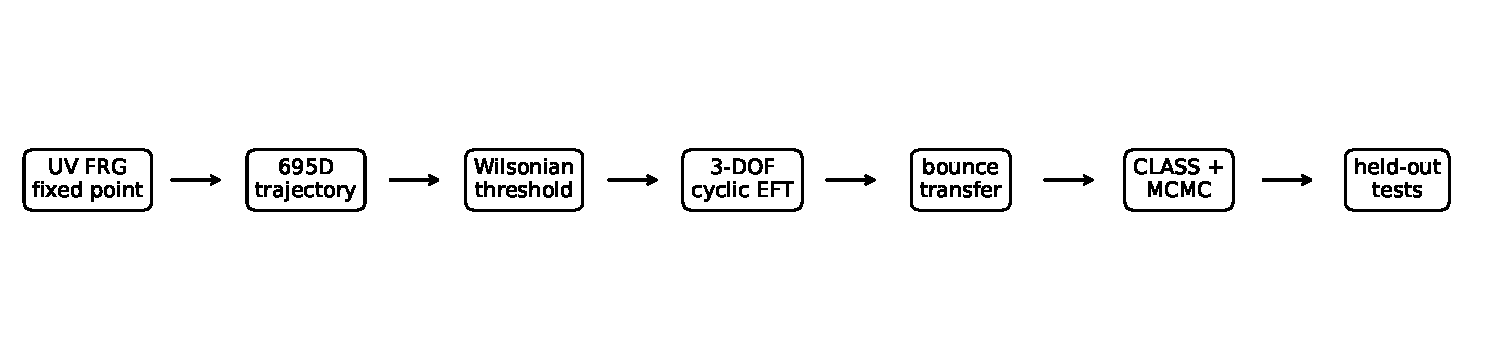
\includegraphics[width=0.96\linewidth]{figures/fig_pipeline.pdf}
\caption{Reproducibility chain used in this work.  Every interface is represented by a frozen numerical authority and an explicit replay step; arrows denote computations rather than logical implications.}
\label{fig:pipeline}
\end{figure}
}{}

\section{Covariant field content and scale-dependent effective action}
\label{sec:theory}

\subsection{Fields, invariants and conventions}

We use metric signature $(-,+,+,+)$ and set $c=\hbar=1$.  The covariant field content consists of the metric $g_{\mu\nu}$, a unit timelike vector $A_\mu$, a scalar temporal field $\phi$, matter fields, and the auxiliary/constraint variables required by the nonlinear Hamiltonian formulation.  The unit condition is imposed with a Lagrange multiplier,
\begin{equation}
 A_\mu A^\mu=-1.
\label{eq:unit}
\end{equation}
The field strength of the vector is
\begin{equation}
 F_{\mu\nu}=\nabla_\mu A_\nu-\nabla_\nu A_\mu,
\end{equation}
and the projector orthogonal to the preferred timelike direction $u^\mu$ is
\begin{equation}
 P^{\mu\nu}=g^{\mu\nu}+u^\mu u^\nu.
\label{eq:projector}
\end{equation}
For the scalar sector we use the dimensionless invariants $\Q$ and $\Y$ employed in the numerical projection.  Their normalization is fixed by the frozen source implementation; operationally, $\Q$ parametrizes the time-like/background scalar derivative and $\Y$ the orthogonal spatial-gradient invariant.  This operational definition is important because the FRG computation is performed directly in the $(\Y,\Q)$ functional space.

A convenient covariant seed action can be written schematically as
\begin{equation}
\begin{split}
S_{\rm seed}=&\int \dd^4x\sqrt{-g}\left[
\frac{\mpl^2}{2}R
-\frac{Z_A}{4}F_{\mu\nu}F^{\mu\nu}
+\mpl^2\cL_{\phi A}(\Y,\Q;K_B,\xi,c_t,\ldots)
+\lambda_A^{(c)}(A_\mu A^\mu+1)
+\cL_m
\right]
+S_{\rm bridge},
\end{split}
\label{eq:seed}
\end{equation}
where $Z_A=1+\alpha_s$ is the transverse vector wave-function coefficient.  The symbol $\lambda_A^{(c)}$ denotes the unit-norm constraint multiplier and must not be confused with the finite potential coupling $\lambda_A$ used in the FRG state vector.  The scalar--vector Lagrangian $\cL_{\phi A}$ is represented non-perturbatively in the retained functions described below rather than by a finite Taylor polynomial.

The Wilsonian alignment term is
\begin{equation}
S_{\rm bridge}=\frac12\int\dd^4x\sqrt{-g}\,
M_A^2(X,\phi)P^{\mu\nu}(A_\mu-u_\mu)(A_\nu-u_\nu).
\label{eq:bridge}
\end{equation}
It is this operator, not the $G(\Q)$ functional channel and not any numerical infrared regulator, that defines the physical transverse mass.  Around the aligned background, the transverse inverse propagator takes the form
\begin{equation}
\Gamma^{(2)}_{A,T}(p)=Z_Ap^2+m_A^2,
\qquad m_A^2\equiv M_A^2(X,\phi).
\label{eq:vectorprop}
\end{equation}

\subsection{Retained functional truncation}

At scale $k$, the effective average action $\Gamma_k$ is represented by the packed state
\begin{equation}
X_k=\big[V(\Q),F(\Y,\Q),g_{\rm fin},H(\Y,\Q),G(\Q),W(\Y,\Q),K(\Y,\Q),U(\Q)\big],
\label{eq:packed}
\end{equation}
with
\begin{equation}
g_{\rm fin}=(\kappa,\xi,c_t,\alpha_s,\lambda_A,w_{\rm Weyl},w_{\rm shear}).
\end{equation}
The one-dimensional functions are $V,G,U$, while $F,H,W,K$ are represented on a two-dimensional $(\Y,\Q)$ grid.  For an $N_Y\times N_Q$ collocation grid, the state-space dimension is
\begin{equation}
N_X=4N_YN_Q+3N_Q+7,
\label{eq:dim}
\end{equation}
so that the $16\times8$ representation has $N_X=567$.  Adding the 128-dimensional bridge sector gives the 695-dimensional source-exact merger used for the threshold trajectory.

The functions $H,W,K$ are defined operationally by finite-momentum projection of the scalar two-point sector.  They multiply the retained $p^4$, $p^6$, and $p^8$ structures, respectively.  This distinction matters: $W$ is a sixth-order scalar projector coefficient, not the vector wave-function factor.  The latter is $Z_A=1+\alpha_s$.

The canonical parts of the corresponding dimensionless flows are
\begin{align}
\partial_t H &=2H+\Q\,\partial_\Q H+4\Y\,\partial_\Y H+\cS_H,\\
\partial_t W &=4W+\Q\,\partial_\Q W+4\Y\,\partial_\Y W+\cS_W,\\
\partial_t K &=6K+\Q\,\partial_\Q K+4\Y\,\partial_\Y K+\cS_K,\\
\partial_t G &=2G+\Q\,\partial_\Q G+\cS_G,
\label{eq:canonicalflows}
\end{align}
where $\cS_i$ denote the projected quantum-source contributions from the Wetterich trace.  The explicit source implementation, including the tensor, scalar, vector, ghost, and constraint contributions, is part of the frozen authority package.

\section{Functional RG construction and UV fixed point}
\label{sec:frg}

\subsection{Wetterich equation and regulator}

The scale dependence is governed by the exact functional equation
\begin{equation}
\partial_t\Gamma_k=\frac12\STr\left[
\left(\Gamma_k^{(2)}+\cR_k\right)^{-1}\partial_t\cR_k
\right],\qquad t=\ln(k/k_0),
\label{eq:wetterich}
\end{equation}
with the supertrace including statistics and internal indices \cite{Wetterich1993,Reuter1998,Saueressig2023}.  The production projection uses an optimized/Litim-type regulator \cite{Litim2001}, harmonic de Donder gauge for the metric fluctuation, and the associated Faddeev--Popov determinant.  The functional domain is
\begin{equation}
0\le \Q\le1.5,\qquad 0\le\Y\le0.3,
\end{equation}
with ascending Chebyshev--Gauss--Lobatto nodes and even-$\Q$ parity where imposed by the source symmetry.

At each collocation node, the functional trace is projected onto the retained operator basis.  The source terms of the $p^4,p^6,p^8$ sector are defined by the corresponding finite-momentum coefficients rather than inferred from canonical scaling.  The production calculation therefore separates the genuine trace source $\cS_i$ from the known transport/canonical part of Eq.~(\ref{eq:canonicalflows}).

\subsection{Fixed-point solve and residuals}

A fixed function $X_*$ satisfies
\begin{equation}
\beta[X_*]=0.
\end{equation}
We solve this system with damped Newton updates,
\begin{equation}
X_{n+1}=X_n-\alpha_n J_n^+\beta(X_n),
\end{equation}
where $J_n$ is the full finite-difference Jacobian, $J_n^+$ is an SVD-regularized pseudoinverse, and $\alpha_n$ is chosen by an Armijo decrease condition.  Fixed points were replayed over multiple resolutions and bridge seeds; an example $16\times8$ solve initialized with a bridge perturbation of $10^{-3}$ converged to an $L_2$ beta residual $2.13\times10^{-7}$, nodewise maximum $9.01\times10^{-8}$, and off-grid residual $4.38\times10^{-8}$.

The older high-resolution fixed-function sector provides an independent resolution benchmark: on a $28\times12$ grid, the retained-sector residuals were
\begin{equation}
\|\beta\|_2=1.838\times10^{-9},\qquad
\|\beta\|_\infty=7.704\times10^{-10},
\end{equation}
with normalized residual $5.145\times10^{-10}$, off-grid residual $3.09\times10^{-10}$, and minimum denominator gap $0.975388$.  These numbers should be interpreted as truncation-internal convergence tests, not as a proof of regulator-independent all-orders asymptotic safety.

A representative reduced fixed-point coordinate set in the gravity/vector subsector is
\begin{equation}
 g_*\simeq0.5824,\qquad
 \lambda_*\simeq0.3348,\qquad
 K_{B*}\simeq0.9298,
\end{equation}
with $\eta_N=-2$ and a small vector-sector anomalous dimension $\eta_B\simeq-0.016$.  Because the apparent count of relevant directions changes when canonical, bridge, and redundancy directions are added or quotiented, we do not promote a single raw $N_{\rm rel}$ to a universal prediction.  The physical stability matrix is instead defined after specifying the retained representation and redundancy prescription,
\begin{equation}
B_{ij}=\left.\frac{\partial\beta_i}{\partial X_j}\right|_{X_*},\qquad
Bv_I=-\theta_Iv_I.
\label{eq:stability}
\end{equation}
This is consistent with the broader asymptotic-safety literature, where stability spectra and almost-Gaussian directions are known to depend sensitively on the projection and the treatment of field redefinitions \cite{Knorr2023,BeckerKurovSaueressig2024,SaueressigSilva2024}.

\subsection{What is and is not claimed}
\IfFileExists{figures/fig_rg_trajectory.pdf}{
\begin{figure}
\centering
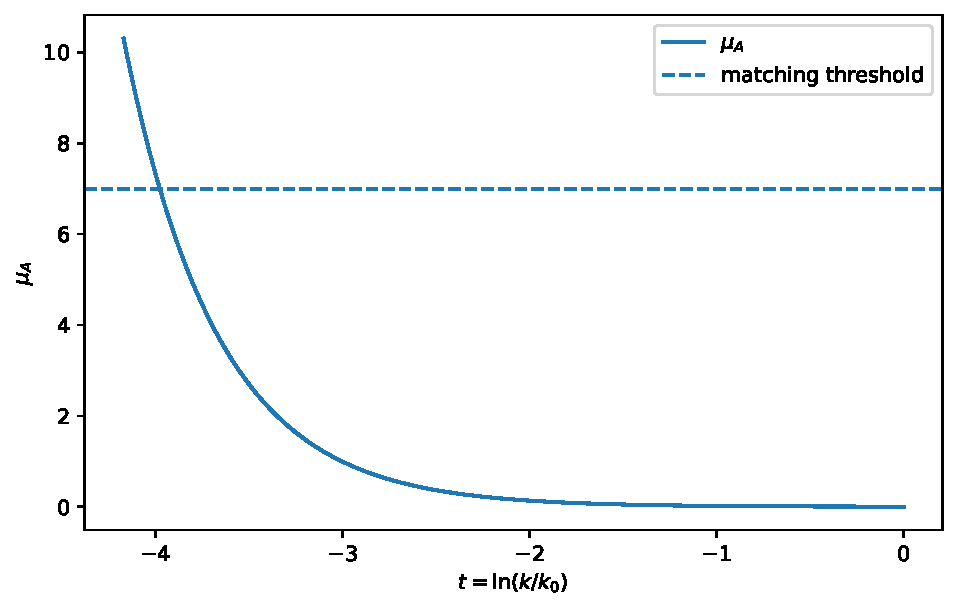
\includegraphics[width=0.90\linewidth]{figures/fig_rg_trajectory.pdf}
\caption{Selected coordinates along the frozen source-exact RG trajectory.  The plotting script reads the released trajectory array directly and performs no smoothing or parameter refit.}
\label{fig:rgtrajectory}
\end{figure}
}{}


The fixed point establishes a non-trivial UV solution of the declared functional system and supplies initial data for the trajectory calculation.  It does not establish regulator-independent all-orders quantum gravity.  A stronger statement would require, at minimum, systematic enlargement of the functional basis, regulator-family stability, and control of the physical quotient of redundant directions.  Our use of ``asymptotically safe'' therefore means ``controlled by an interacting fixed point within the source-explicit truncation studied here.''

\section{Wilsonian heavy-vector threshold and matching}
\label{sec:wilson}

\subsection{Physical threshold variable}

From Eq.~(\ref{eq:vectorprop}) the dimensionless pole-mass variable is
\begin{equation}
\mu_A(k)=\frac{m_A^2(k)}{Z_A(k)k^2}.
\label{eq:mu}
\end{equation}
With anomalous-dimension convention
\begin{equation}
\eta_A=-\partial_t\ln Z_A,
\end{equation}
the canonical part of its flow is
\begin{equation}
\beta_{\mu_A}=(-2+\eta_A)\mu_A+\Delta\beta_{\mu_A},
\label{eq:betamu}
\end{equation}
where $\Delta\beta_{\mu_A}$ is evaluated from the source-exact trace.  In a simplified constant-mass check the vector threshold contribution reduces to a decoupling form proportional to $2\mu_A/(1+\mu_A)^2$, but the production trajectory uses the coupled 695-dimensional flow rather than this approximation.

\subsection{Coupled UV-to-threshold trajectory}

Starting near the fixed point, the 567-dimensional functional sector and 128-dimensional bridge sector are integrated simultaneously.  The threshold authority uses two stiff solvers, Radau and BDF, as a parity check.  At $\mu_A=7$ the canonical handoff state is
\begin{align}
 t_{\rm match}&=-3.97664237,\\
 k_{\rm match}&=1.87484842\times10^{-2}\mpl,\\
 Z_A&=1.000075,\\
 m_A^2&=2.46072415\times10^{-3}\mpl^2,
\end{align}
with minimum denominator gaps
\begin{equation}
\Delta_T=0.645538,\qquad \Delta_S=0.950492,\qquad \Delta_A=8.000600.
\end{equation}
The full-state defect measured against the differential equation satisfies
\begin{equation}
\max_i|\dot X_i-\beta_i(X)|=7.68\times10^{-7},\qquad
\|\dot X-\beta\|_2=9.14\times10^{-6},
\end{equation}
and the Radau--BDF state disagreement is $6.22\times10^{-7}$ componentwise at maximum and $7.40\times10^{-6}$ in $L_2$ norm.

\subsection{Derivative expansion of the heavy propagator}

For momenta below the heavy-vector pole, the tree-level exchange kernel has the generic structure
\begin{equation}
\cK_{\rm full}(p^2)=-\frac{g_B^2p^2}{Z_Ap^2+m_A^2}.
\label{eq:kernel}
\end{equation}
For $Z_Ap^2/m_A^2<1$,
\begin{equation}
\cK_{\rm full}(p^2)=
-\frac{g_B^2}{m_A^2}p^2
+\frac{g_B^2Z_A}{m_A^4}p^4
-\frac{g_B^2Z_A^2}{m_A^6}p^6
+\frac{g_B^2Z_A^3}{m_A^8}p^8
+\cO(p^{10}).
\label{eq:derivativeexpansion}
\end{equation}
The $p^4,p^6,p^8$ terms shift the retained $H,W,K$ Wilson coefficients.  A degree-eight projection evaluated on 400 dense points yields normalized maximum residuals
\begin{equation}
R_{\rm inv}=1.23\times10^{-7},\quad
R_{\rm tree}=9.84\times10^{-7},\quad
R_{\rm Hess}=9.25\times10^{-16}.
\label{eq:projectionres}
\end{equation}

\subsection{Coefficient shifts versus matching error}
\IfFileExists{figures/fig_matching_ledger.pdf}{
\begin{figure}
\centering
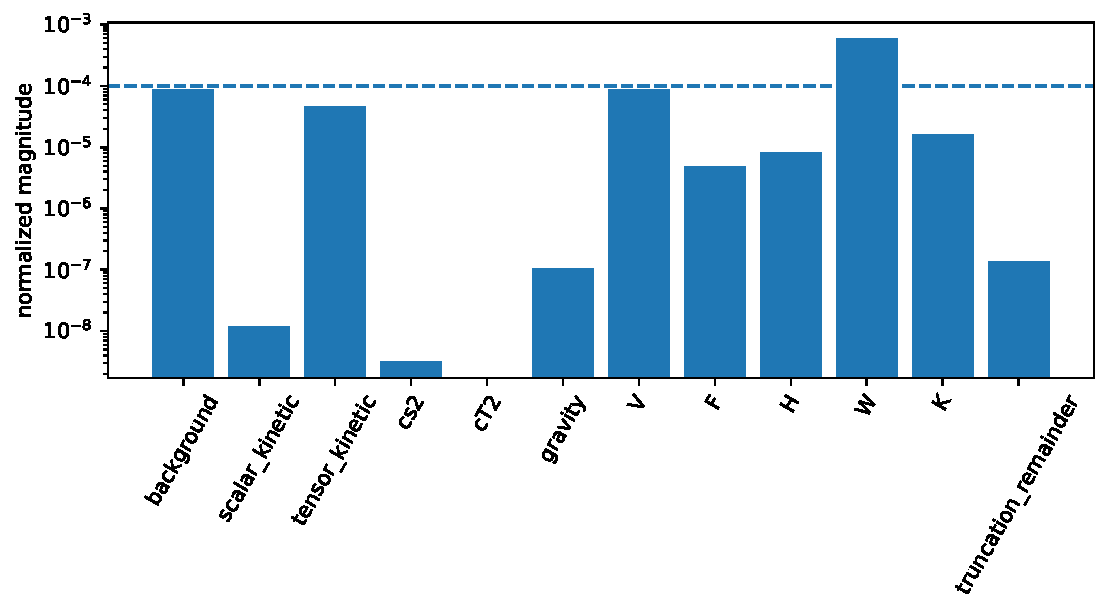
\includegraphics[width=0.90\linewidth]{figures/fig_matching_ledger.pdf}
\caption{Strict Wilsonian matching ledger.  Raw Wilson-coefficient shifts are displayed separately from represented post-match residuals and from the unrepresented truncation remainder.  The horizontal line marks the predeclared $10^{-4}$ matching-error threshold.}
\label{fig:matchingledger}
\end{figure}
}{}


A central bookkeeping point is that a Wilson coefficient shift is not itself a matching error.  Let $c_i^-$ denote the pre-threshold IR coefficients and $\Delta c_i$ the shifts generated by integrating out the vector.  The matched EFT is
\begin{equation}
\Gamma_{\rm EFT}[c_i^+],\qquad c_i^+=c_i^-+\Delta c_i.
\end{equation}
For projector $\Pi_i$, the represented post-match residual is
\begin{equation}
r_i=\frac{\Pi_i\Gamma_{\rm full}-\Pi_i\Gamma_{\rm EFT}[c^+]}{N_i},
\label{eq:rmatch}
\end{equation}
where $N_i$ is the predeclared channel normalization.  The matching error is then
\begin{equation}
R_{\rm match}=\max\left(\max_i|r_i|,R_{\rm unrepresented}\right),
\label{eq:Rmatch}
\end{equation}
not $\max_i|\Delta c_i|$.  In the canonical $\mu_A=7$ projection the largest normalized retained coefficient displacement occurs in the $W$ channel, $|\Delta W|_{\rm norm}=5.8868\times10^{-4}$.  The reported omitted-derivative remainder after the retained Wilson shifts is $5.21\times10^{-5}$ and the dense projector remainder is $9.84\times10^{-7}$.  Thus the coefficient displacement must be listed in the matching ledger, but it is not counted as an unabsorbed EFT error.  This distinction is essential when applying the strict $10^{-4}$ post-match-error target.

Below the matching scale, the explicit vector trace and bridge-state dimensions are removed from the running state.  Their effects remain only in the matched Wilson coefficients.  This realizes the physical decoupling of the heavy vector rather than merely suppressing it numerically.

\section{Infrared cyclic cosmology and perturbations through the bounce}
\label{sec:cyclic}

\subsection{Background equations}

After matching, the light gravitational sector contains the metric and one physical scalar mode.  On a spatially flat FLRW background,
\begin{equation}
\dd s^2=-\dd t^2+a^2(t)\delta_{ij}\dd x^i\dd x^j,
\end{equation}
the constraint and evolution equations may be written as
\begin{align}
3\mpl^2H^2 &= \rho_r+\rho_b+\rho_{\rm eff},\label{eq:friedmann}\\
-2\mpl^2\dot H &= (\rho_r+p_r)+(\rho_b+p_b)+(\rho_{\rm eff}+p_{\rm eff}),\label{eq:raych}\end{align}
where $\rho_{\rm eff}$ and $p_{\rm eff}$ are obtained directly from the matched scalar-temporal action and its constraint solution.  No cold-particle dark-matter density is introduced in the production CLASS branch.  The background is evolved in a variable regular at $H=0$, allowing the turnaround and bounce to be treated as regular roots of the constrained system rather than endpoints of separate analytic branches.

The frozen cyclic solution has a minimum scale factor
\begin{equation}
a_{\min}=1.074131848\times10^{-13}
\end{equation}
and a future maximum scale factor $a_{\max}\simeq2.06$ in the normalization $a_0=1$.  The likelihood calculation uses the expanding post-bounce branch, while the through-bounce campaign described below independently verifies that the perturbation state can be propagated from the contracting side into the CLASS branch.

\subsection{Constraint reduction at quadratic order}

The scalar perturbations are introduced in the usual scalar decomposition of the metric and matter variables.  Lapse, shift, and nondynamical vector/scalar combinations are eliminated by their constraint equations before identifying the physical scalar.  The reduced quadratic scalar action can be represented as
\begin{equation}
S_s^{(2)}=\frac12\int\dd t\,\dd^3k\left[
Q_s(t,k)|\dot q_s|^2-Q_s(t,k)\omega_s^2(t,k)|q_s|^2
\right],
\label{eq:scalarquad}
\end{equation}
where the retained derivative expansion implies
\begin{equation}
\omega_s^2=c_{s,2}^2\frac{k^2}{a^2}
+c_{s,4}\frac{k^4}{a^4M_*^2}
+c_{s,6}\frac{k^6}{a^6M_*^4}
+c_{s,8}\frac{k^8}{a^8M_*^6}.
\label{eq:omegas}
\end{equation}
The tensor action takes the analogous form
\begin{equation}
S_T^{(2)}=\frac18\sum_{\lambda=+,\times}\int\dd t\,\dd^3k\,
a^3Q_T\left[|\dot h_\lambda|^2-\omega_T^2|h_\lambda|^2\right].
\label{eq:tensorquad}
\end{equation}
The numerical stability audit tests positivity of the physical kinetic eigenvalues and of $\omega^2$ over the entire tested time--$k$ domain; it does not infer stability solely from the background equations.

\subsection{Regular canonical variables and transfer matrix}

Variables containing explicit $H^{-1}$ or $H^{-2}$ factors are unsuitable at the bounce.  The regular canonical representation used in the replay can be chosen proportional to
\begin{equation}
(q_s,p_s)=(\Phi,a^5\dot\Phi),\qquad
(q_T,p_T)=(h,a^3\dot h),
\label{eq:canonicalvars}
\end{equation}
with normalization fixed by the reduced quadratic action.  For each Fourier mode the first-order system is
\begin{equation}
\dot{\bm X}=A_k(t)\bm X,
\qquad \bm X=(q,p)^T.
\label{eq:firstorder}
\end{equation}
Integrating two linearly independent basis states from $t_-$ to $t_+$ defines the bounce transfer matrix
\begin{equation}
\bm X(t_+)=\cT(k)\bm X(t_-).
\end{equation}
Canonical evolution requires
\begin{equation}
\cT^T J\cT=J,\qquad
J=\left(\begin{array}{cc}0&1\\-1&0\end{array}\right),
\label{eq:symplectic}
\end{equation}
which is used as a numerical diagnostic rather than imposed algebraically on the output.

The production through-bounce campaign used 120 modes and multiple stiff/nonstiff solvers.  An independent recomputation obtained a maximum symplectic residual $5.20\times10^{-13}$ and a Radau--DOP853 transfer disagreement $2.79\times10^{-11}$.  On observable scales the scalar transfer is non-trivial but effectively scale independent; the diagonal transfer amplitude is
\begin{equation}
T_{s,11}\simeq T_{s,22}\simeq0.93968314,
\end{equation}
and the curvature-power mapping is
\begin{equation}
\frac{P_{\cal R}^{+}}{P_{\cal R}^{-}}=0.8830044.
\label{eq:Prtransfer}
\end{equation}
The tensor transfer is consistent with the identity at the tested precision.  Consequently, for the observable branch the principal bounce effect is an amplitude mapping rather than a new oscillatory or strongly scale-dependent primordial feature.  The MCMC parameter $A_s$ is therefore interpreted as the post-bounce amplitude used by CLASS; Eq.~(\ref{eq:Prtransfer}) maps it to the corresponding pre-bounce normalization.

\section{Boltzmann implementation and cosmological inference}
\IfFileExists{figures/fig_bounce_transfer.pdf}{
\begin{figure}
\centering
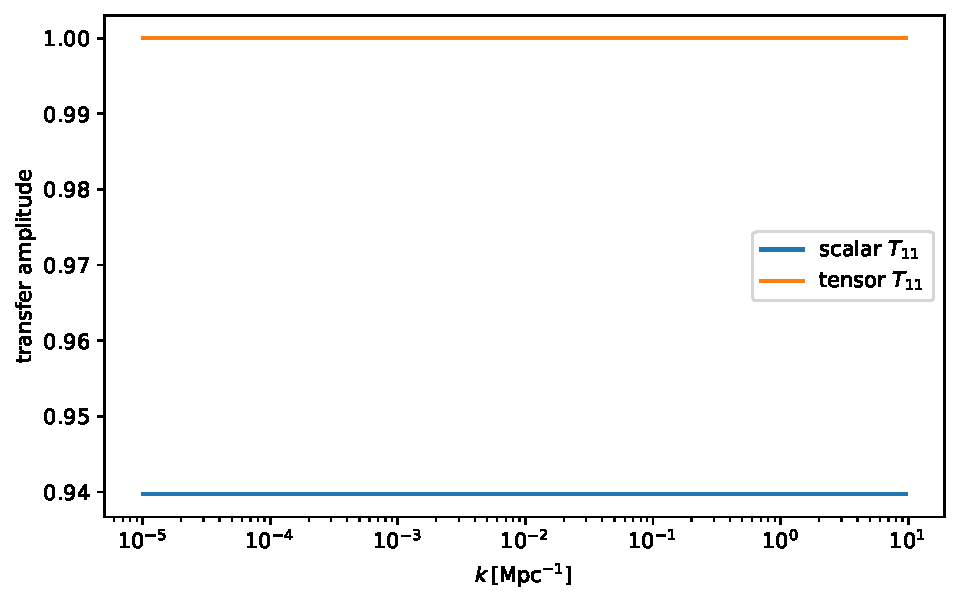
\includegraphics[width=0.90\linewidth]{figures/fig_bounce_transfer.pdf}
\caption{Scalar and tensor through-bounce transfer diagnostics as functions of comoving wavenumber.  Final publication curves are regenerated from the frozen transfer-matrix arrays.}
\label{fig:bouncetransfer}
\end{figure}
}{}

\label{sec:observations}

\subsection{CLASS implementation}

The post-bounce equations are implemented in a frozen CLASS branch.  The production source modifies the background and perturbation sectors while retaining the standard photon, baryon, neutrino, recombination, transfer, and harmonic infrastructure of CLASS \cite{BlasLesgourguesTram2011}.  The cosmological inference uses Cobaya \cite{TorradoLewis2021}.  The baseline sampled coordinates are
\begin{equation}
\{H_0,\omega_b,\omega_{\rm eff},s_4,n_s,A_s,\tau_{\rm reio},A_{\rm Planck}\},
\end{equation}
where $\omega_{\rm eff}$ is the effective dark-sector-like density generated by the matched scalar-temporal sector and $s_4$ is the active cyclic-shape coordinate.  The remaining shape coefficients and microscopic parameters are frozen by the theory authority rather than refitted to held-out data.

The production chain uses the frozen Planck-2018 CMB, DESI BAO, and Pantheon+ supernova likelihood stack, with no SH0ES local-$H_0$ likelihood in the chain used here \cite{Planck2018VI,DESI2024BAO,DESI2025DR2BAO,BroutPantheonPlus2022}.  The four-chain run contains 49,309 stored rows.  Applying a 30\% burn-in in the independent replay leaves 34,518 rows and a Kish effective sample size $N_{\rm eff}=30,537.9$.  The maximum replayed Gelman--Rubin statistic is
\begin{equation}
\max(R-1)=0.005105<0.01.
\end{equation}

\begin{table}[t]
\caption{Posterior means and standard deviations from the independently replayed raw chains.  The numerical values refer to the frozen production authority.}
\label{tab:posterior}
\begin{indented}
\item[]\begin{tabular}{@{}lll}
\br
Parameter & Mean & Standard deviation\\
\mr
$H_0$ [km s$^{-1}$ Mpc$^{-1}$] & 68.6219 & 0.3012\\
$\omega_b$ & 0.0225106 & 0.0001258\\
$\omega_{\rm eff}$ & 0.118325 & 0.000629\\
$s_4$ & 0.357260 & 0.056026\\
$n_s$ & 0.968479 & 0.003182\\
$A_s$ & $2.10576\times10^{-9}$ & $2.859\times10^{-11}$\\
$\tau_{\rm reio}$ & 0.057578 & 0.006661\\
$A_{\rm Planck}$ & 1.00073 & 0.00245\\
\br
\end{tabular}
\end{indented}
\end{table}

The independently reconstructed best-fit cyclic point has
\begin{equation}
H_0=68.7803,\quad \omega_b=0.0225283,\quad
\omega_{\rm eff}=0.118347,\quad s_4=0.434373,
\end{equation}
\begin{equation}
n_s=0.968976,\quad A_s=2.09693\times10^{-9},\quad
\tau_{\rm reio}=0.05624.
\end{equation}
At this point the Boltzmann solver gives $\sigma_8=0.82015$, $\Omega_m=0.29779$ and $S_8=0.81713$.  The matched $\LCDM$ comparator gives $\sigma_8=0.82026$, $\Omega_m=0.29730$ and $S_8=0.81655$.

\subsection{Held-out lensing and growth}
\IfFileExists{figures/fig_mcmc_convergence.pdf}{
\begin{figure}
\centering
\includegraphics[width=0.90\linewidth]{figures/fig_mcmc_convergence.pdf}
\caption{Final-chain convergence diagnostics.  This figure is intentionally absent from draft builds until the production chains reach the frozen stopping criterion.}
\label{fig:mcmcconv}
\end{figure}
}{}

\IfFileExists{figures/fig_heldout_delta_chi2.pdf}{
\begin{figure}
\centering
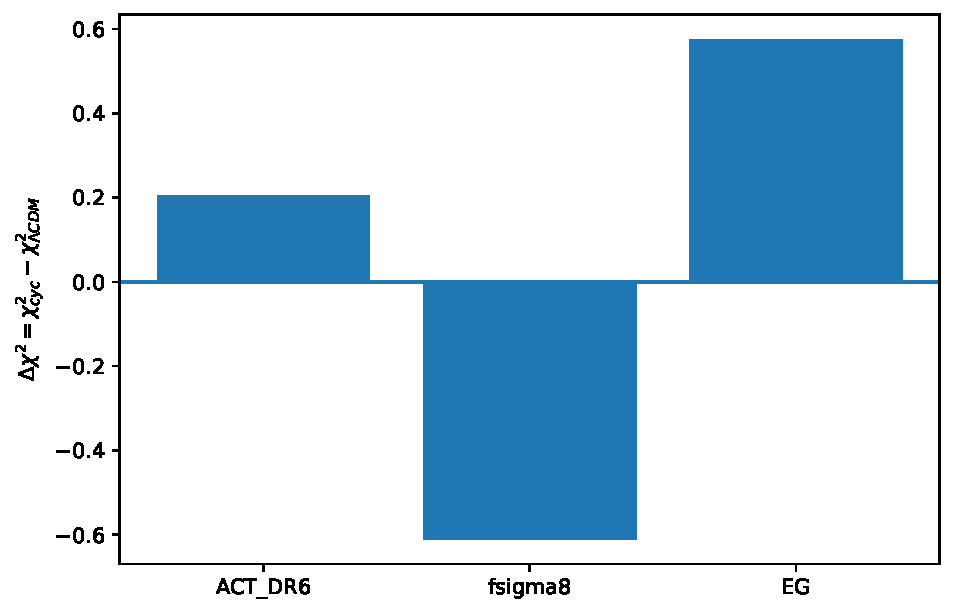
\includegraphics[width=0.90\linewidth]{figures/fig_heldout_delta_chi2.pdf}
\caption{Held-out likelihood contributions relative to the matched $\Lambda$CDM comparator, regenerated from the frozen final-chain best-fit theory.  Positive values favour neither model by themselves; the sign convention is $\Delta\chi^2=\chi^2_{\rm cyc}-\chi^2_{\Lambda\rm CDM}$.}
\label{fig:heldout}
\end{figure}
}{}


The held-out validation uses ACT DR6 CMB lensing, a twelve-point $f\sigma_8$ compilation, and eight $E_G$ measurements.  ACT DR6 is evaluated with the official likelihood, including its covariance and likelihood corrections \cite{MadhavacherilACT2023}.  The result of the independent replay is
\begin{align}
\chi^2_{\rm ACT,cyc}&=18.305377,\\
\chi^2_{\rm ACT,\LCDM}&=18.099977,\\
\Delta\chi^2_{\rm ACT}&=+0.205400.
\end{align}
For lens-only ACT DR6, the difference is $\Delta\chi^2=-0.337181$.

For the growth measurements,
\begin{align}
\chi^2_{f\sigma_8,{\rm cyc}}&=9.429533, &
\chi^2_{f\sigma_8,\LCDM}&=10.039742,\\
\chi^2_{E_G,{\rm cyc}}&=5.549303, &
\chi^2_{E_G,\LCDM}&=4.974539.
\end{align}
Thus the combined 30-point held-out statistic is
\begin{equation}
\chi^2_{\rm cyc}=33.284213,\qquad
\chi^2_{\LCDM}=33.114258,
\end{equation}
with
\begin{equation}
\Delta\chi^2_{\rm heldout}=+0.169955.
\label{eq:heldout}
\end{equation}
The appropriate interpretation is compatibility, not evidence of superiority: $|\Delta\chi^2|\ll1$ for this validation vector.

Recent CMB-lensing and weak-lensing datasets provide additional stringent tests \cite{PanSPT2023,AmonDES2022,SeccoDES2022,DalalHSC2023,LiHSC2023}.  We do not promote nonlinear galaxy-scale or cosmic-shear likelihoods to fundamental tests unless the required nonlinear mapping of the matched theory is independently established.  In particular, the present source authority validates the linear/quasi-linear cosmological regime; it does not justify inserting a GR-calibrated nonlinear fitting function and relabelling it as a prediction of the fundamental theory.

\subsection{Posterior-predictive bookkeeping note}

A reciprocal replay exposed a posterior-predictive bookkeeping discrepancy: an archived DAWN aggregate reports $S_8=0.80896\pm0.00787$, whereas an ASUS propagation reports $S_8=0.81883\pm0.00829$.  The difference is too large to label as Monte-Carlo noise.  Inspection shows that the two calculations did not use an identical immutable posterior-sample manifest.  We therefore do not select either mean for the final paper at this stage.  At final-chain freeze, both machines will propagate the same cryptographically hashed list of chain-file/row identifiers through the same hashed CLASS source and compare $S_8$ sample by sample.  Until that reconciliation passes, no posterior-predictive $S_8$ aggregate is used in a headline conclusion.  The likelihood-level ACT, $f\sigma_8$, and $E_G$ replay results are a separate calculation and agree between machines at the $10^{-3}$--$10^{-4}$ level in $\Delta\chi^2$ for the validation snapshot.

\section{Reproducibility architecture and reciprocal replay}
\label{sec:repro}

A central design objective of this work is that numerical authority is carried by source, raw arrays, hashes, and deterministic replay scripts rather than by prose certificates.  The observational authority archive used in the reciprocal replay has SHA-256
\begin{verbatim}
8a5817e4200b9a790dfd61d62753ebeed692af8ccb6945637aa6008dab6c91da
\end{verbatim}
The exact CLASS executable and principal modified source files used by the replay have hashes
\begin{verbatim}
CLASS executable:
8ddc0ec60c2fe6ff86ab2e2f1dd35e259dfbcabfe00f49defcf43081a4ac183f
background.c:
5015272d0d1f9eb186aaaca38531e7775782b6de2605d60c5c02bb746511d2b4
perturbations.c:
60f801b9182eb7f6788a21b2074be24532d4b4a2c26e0574b537a582fa605e37
thermodynamics.c:
b4015ba4e673022a7b2087bc506279f3de2abc1ff5374c4ab6a67309726a6d5f
\end{verbatim}
The source-exact merger archive is likewise frozen with its own SHA-256 manifest.  Reproduction is considered successful only when the archive checksum, internal source checksums, numerical tolerances, and declared solver versions are verified before evaluating a scientific gate.

The reciprocal validation is intentionally asymmetric.  The perturbation/bounce result was independently recomputed on the cosmology machine from the frozen theory authorities, whereas the cosmology likelihood result was independently replayed on the theory machine from raw chains and the official likelihood modules.  The latter replay reconstructed all critical parameter points, evaluated ACT DR6 directly through the official likelihood interface, and independently recomputed the $f\sigma_8$ and $E_G$ residual vectors.  The final combined held-out discrepancy between the two machines was $4.74\times10^{-4}$ in $\Delta\chi^2$.

This procedure is stronger than rerunning the same summary script on a second host, but it is not equivalent to an independent external-group replication.  All machines, design choices, and frozen authorities remain part of the same research programme.  External reproduction is therefore an explicit next-stage falsification criterion.

\section{Discussion: what would constitute a paradigm shift?}
\label{sec:discussion}

The construction combines several elements that are usually studied separately: a non-perturbative UV fixed point, a resolved Wilsonian threshold, a three-light-degree-of-freedom IR theory, a nonsingular cyclic background, a calculated perturbation transfer through the bounce, a Boltzmann implementation, MCMC inference, held-out lensing/growth tests, and reciprocal source-level replay.  If this chain survives external reconstruction, larger FRG truncations, regulator changes, nonlinear structure calculations, and independent cosmological likelihoods, the conceptual implication would be substantial.  It would show that dark-sector-like cosmological phenomenology can emerge as an IR description of a gravitational RG trajectory with an explicitly decoupled heavy sector, rather than being postulated as a separate particle component.

That possibility is reasonably described as \emph{paradigm-changing}.  It is not yet scientifically justified to describe the theory as \emph{the new paradigm}.  A paradigm in the Kuhnian or practical scientific sense is established by community-level explanatory success, independent replication, predictive novelty, and comparative performance over time.  The present work supplies a candidate architecture and an unusually direct reproduction target.  Its credibility should increase or decrease according to how those tests turn out.

The recent literature makes this standard particularly important.  Modern asymptotic-safety studies emphasize the trajectory from fixed-point data to physical predictions rather than the fixed point alone \cite{SaueressigSilva2024}; canonical and Lorentzian formulations stress the nontrivial role of physical observables and gauge reduction \cite{DAngelo2024,Thiemann2024}; and current large-scale-structure datasets make percent-level tests of lensing and growth routine \cite{DESI2024BAO,DESI2025DR2BAO,MadhavacherilACT2023,DalalHSC2023}.  A candidate fundamental cosmology should therefore be judged by whether it closes these interfaces transparently.

An alternative microscopic gauge-geometric programme based on compact $U(1)$ dimension-field symmetries is also being investigated \cite{PartanenTulkki2025}.  That programme is not used as an assumption in the present paper.  In current cross-comparisons it is treated as an independent candidate microscopic realization whose operator map, stability spectrum, and UV-to-IR trajectory must agree before an equivalence claim is made.

\section{Limitations and falsifiability}
\label{sec:limits}

The principal limitations are explicit.

First, the UV result is truncation dependent.  The retained functional space is substantially larger than a polynomial Einstein--Hilbert truncation, but it is finite.  Regulator-family and operator-basis enlargements remain necessary tests of universality.  A persistent loss of the interacting fixed point, physical denominator gap, or UV-critical surface under systematic enlargement would falsify the present UV interpretation.

Second, the heavy-vector matching is controlled only over the declared derivative range.  The strict matching error must be evaluated after retained Wilson shifts, as in Eq.~(\ref{eq:Rmatch}); a coefficient displacement is not an error.  If an independent matching ledger finds a genuine post-fit residual exceeding $10^{-4}$ in a represented physical channel, the canonical handoff used here would fail its own declared criterion.

Third, the nonlinear galaxy regime is not closed from first principles in this paper.  Strong-lensing systems and small-scale cosmic shear probe momenta and environments for which an ab initio nonlinear completion of the matched EFT is required.  A GR-calibrated halo or nonlinear transfer function cannot be silently imported as a prediction of the present theory.

Fourth, the reciprocal machine replays are internal independent calculations, not external replication.  A decisive test is whether an unaffiliated group can reproduce: (i) the source-exact fixed point, (ii) the physical stability spectrum, (iii) the 695-dimensional trajectory to $\mu_A=7$, (iv) the derivative matching, (v) the through-bounce transfer, and (vi) the held-out likelihoods from the public package.

Finally, the observational result in Eq.~(\ref{eq:heldout}) is intentionally modest.  The held-out data do not distinguish the cyclic theory from the matched $\LCDM$ comparator at a meaningful level.  Future discrimination must come from observables where the theories make genuinely separated predictions, not from reinterpreting a near-zero $\Delta\chi^2$.

\section{Conclusions}
\label{sec:conclusions}

We have constructed and numerically connected a chain from an interacting FRG fixed point to a low-energy cyclic cosmology.  The construction is source explicit: the UV functional state, finite-momentum projectors, physical heavy-vector mass, threshold variable, matching coefficients, bounce transfer, Boltzmann source, MCMC chains, and held-out likelihood interfaces are all separately frozen and replayable.

Within the declared truncation, the fixed-point equations admit converged non-trivial solutions, and the coupled 695-dimensional source-exact flow reaches a controlled heavy-vector threshold with positive propagator gaps and solver parity.  Integrating out the vector produces a derivative expansion captured through $p^8$; after separating Wilson-coefficient shifts from post-fit errors, the reported omitted derivative remainder is below the predeclared $10^{-4}$ target.  The resulting IR theory contains three light propagating modes.  Scalar and tensor perturbations propagate through the bounce with finite, symplectic transfer matrices, and an independent recomputation reproduces the scalar amplitude map and CLASS handoff.

Cosmological chains converge under an independent raw-chain analysis.  Held-out ACT DR6 lensing, $f\sigma_8$, and $E_G$ measurements give a combined $\Delta\chi^2=+0.170$ relative to a matched $\LCDM$ comparator, demonstrating compatibility rather than preference.  The strongest result of the present work is therefore not a claimed statistical victory over $\LCDM$, but the closure of a reproducible theory-to-data pipeline spanning scales that are usually treated in separate effective descriptions.

Whether this becomes a paradigm shift is an empirical and community question.  The paper is written so that the answer need not depend on trust in the authors' interpretation: the core calculations can be rerun, the matching definitions can be challenged, and the theory can be falsified at each interface.  External reproduction and systematic truncation enlargement are now the decisive tests.

\ack
The author acknowledges the developers of CLASS, Cobaya, ACT DR6 likelihood software, and the collaborations that released the cosmological data used in this work.  No external funding was received for this research.  This theoretical/computational study involved no human participants or animal experiments.

\section*{Data and code availability}
The public reproducibility repository is structured to contain the exact manuscript source, BibTeX database, plotting and audit scripts, SHA-256 manifests, modified CLASS source, final raw MCMC chains, likelihood configuration files, and deterministic replay instructions.  Large frozen authority archives may be deposited as versioned release assets or in a DOI-backed archival service, with hashes recorded in the repository.  The repository/DOI identifiers will be inserted here only after the final production-chain freeze and immutable release are created.  No unpublished private data are required for the intended reproduction workflow.

\appendix

\section{Constraint counting and the microscopic-to-IR degree-of-freedom reduction}
\label{app:constraints}

The nonlinear microscopic constrained system is represented on a 42-dimensional phase space with 24 constraints.  In the source authority, six constraints are first class and eighteen are second class.  Dirac counting gives
\begin{equation}
N_{\rm dof}=\frac{42-2N_{\rm FC}-N_{\rm SC}}{2}
=\frac{42-12-18}{2}=6.
\label{eq:dof6}
\end{equation}
The rank-18 second-class block has been checked numerically on deterministic generic algebraic patches, and the expected first-class null directions are independently identified.  This is numerical generic-patch evidence rather than a general symbolic theorem.  The result is compatible with the six nonlinear degrees of freedom found in the Hamiltonian analysis of AeST-like scalar--vector systems \cite{BatakiSkordisZlosnik2024}.

Equation~(\ref{eq:dof6}) does not contradict the three-light-mode statement used in the IR cosmology.  Above the Wilsonian threshold, the six physical modes include the heavy vector sector.  At $\mu_A\gg1$ the transverse vector pole lies above the running scale.  Integrating it out removes the corresponding explicit dynamical coordinates from the IR state and transfers their low-energy effect to local Wilson coefficients.  The matched light theory therefore propagates two tensor polarizations and one scalar mode.  The distinction is between the degree count of the microscopic constrained system and the degree count of the low-energy propagating spectrum.

\section{Functional projection and collocation details}
\label{app:projection}

Let $\{\Q_j\}_{j=1}^{N_Q}$ and $\{\Y_i\}_{i=1}^{N_Y}$ denote ascending CGL nodes mapped to the physical domains.  For a two-dimensional functional $f(\Y,\Q)$ we store
\begin{equation}
f_{ij}=f(\Y_i,\Q_j)
\end{equation}
and use the spectral differentiation matrices $D_Y,D_Q$ to evaluate the canonical transport pieces.  Off-grid interpolation uses the corresponding barycentric representation.  A fixed-point residual is reported in three forms,
\begin{align}
R_2&=\left(\sum_a\beta_a^2\right)^{1/2},\\
R_\infty&=\max_a|\beta_a|,\\
R_{\rm norm}&=\max_a\frac{|\beta_a|}{1+|X_a|},
\end{align}
with an additional deterministic off-grid residual evaluated away from the collocation nodes.

Finite-momentum projection evaluates the two-point kernels at a predeclared set of momenta and extracts polynomial coefficients through the retained order.  A generic even expansion is
\begin{equation}
\Gamma_k^{(2)}(p)=c_0+c_2p^2+c_4p^4+c_6p^6+c_8p^8+\cO(p^{10}).
\end{equation}
The $c_4,c_6,c_8$ pieces define the operational $H,W,K$ channels.  This projector definition avoids assigning a unique covariant monomial to a coefficient when integrations by parts or field redefinitions would make such an assignment basis dependent.

\section{Source-exact threshold flow and solver parity}
\label{app:trajectory}

The merger ODE is
\begin{equation}
\frac{\dd X}{\dd t}=\beta(X),\qquad X\in\mathbb R^{695}.
\end{equation}
The trajectory is integrated independently with implicit Radau and BDF methods.  For a checkpoint $t_j$, define the solver parity metric
\begin{equation}
R_{\rm AB}(t_j)=\frac{\|X_A(t_j)-X_B(t_j)\|_2}{\max(1,\|X_A(t_j)\|_2)}.
\end{equation}
The differential-equation defect is evaluated without using the solver's local error estimate,
\begin{equation}
D(t_j)=\left\|\frac{\dd X}{\dd t}\bigg|_{\rm reconstructed}-\beta[X(t_j)]\right\|.
\end{equation}
This distinction is important: a small stepper error is not by itself evidence that the integrated path solves the intended beta system.

The physical threshold is located by root finding on
\begin{equation}
f(t)=\mu_A(t)-7.
\end{equation}
No coupling is retuned at the crossing.  The full state at the root is serialized before any low-energy projection is performed.

\section{Wilsonian matching ledger}
\label{app:matching}

For each physical projection channel $i$ we distinguish three quantities:
\begin{enumerate}
\item the raw Wilson-coefficient displacement $\Delta c_i$;
\item the represented post-match residual $r_i$ after the coefficient is shifted;
\item the unrepresented truncation remainder $R_{\rm trunc}$ from terms outside the retained basis.
\end{enumerate}
The numerical handoff reports the channel diagnostics
\begin{center}
\begin{tabular}{lc}
\br
Channel diagnostic & normalized value\\
\mr
background & $8.6127\times10^{-5}$\\
scalar kinetic & $1.1920\times10^{-8}$\\
tensor kinetic & $4.6429\times10^{-5}$\\
$c_s^2$ & $3.1547\times10^{-9}$\\
$c_T^2$ & $0$\\
gravity & $1.0335\times10^{-7}$\\
$V$ & $8.6075\times10^{-5}$\\
$F$ & $4.7883\times10^{-6}$\\
$H$ & $8.2435\times10^{-6}$\\
$W$ coefficient displacement & $5.8868\times10^{-4}$\\
$K$ & $1.6229\times10^{-5}$\\
dense projector remainder & $9.8401\times10^{-7}$\\
\br
\end{tabular}
\end{center}
The table records the working classification of the $W$ entry as a retained coefficient displacement.  Before submission this classification is recomputed from the raw full-theory and matched-EFT projector values using the released strict-ledger script.  The independent omitted-derivative estimate is $R_{\rm trunc}=5.21\times10^{-5}$.  The canonical handoff is declared to pass the strict gate only if the recomputed represented residuals and unrepresented remainder satisfy $R_{\rm match}<10^{-4}$ without changing the threshold.

\section{Through-bounce transfer derivation}
\label{app:bounce}

After eliminating constraints, each physical perturbation sector is written in first-order Hamiltonian form,
\begin{equation}
\dot{\bm X}=A(t,k)\bm X.
\end{equation}
Let $\bm e_1=(1,0)^T$ and $\bm e_2=(0,1)^T$ be basis vectors at $t_-$.  Evolving each vector to $t_+$ gives
\begin{equation}
\cT(k)=\left(\begin{array}{cc}
q_1(t_+) & q_2(t_+)\\
p_1(t_+) & p_2(t_+)
\end{array}\right).
\end{equation}
The Wronskian/symplectic residual is
\begin{equation}
R_J(k)=\|\cT^TJ\cT-J\|_F.
\end{equation}
A second solver independently generates $\cT_B$, with
\begin{equation}
R_{\rm solver}(k)=\frac{\|\cT_A-\cT_B\|_F}{\max(1,\|\cT_A\|_F)}.
\end{equation}
The scale-dependence diagnostic is
\begin{equation}
R_k=\max_{k\in K_{\rm obs}}\frac{\|\cT(k)-\cT(k_{\rm ref})\|_F}
{\max(1,\|\cT(k_{\rm ref})\|_F)}.
\end{equation}
The observable scalar transfer is classified as scale-independent and nontrivial when $R_k$ remains below the numerical tolerance while $\|\cT-I\|$ does not.

\section{Boltzmann and likelihood reproduction protocol}
\label{app:likelihood}

A complete likelihood replay proceeds in the following fixed order.
\begin{enumerate}
\item Verify the authority archive SHA-256 and the internal file manifest.
\item Read the four raw chains; apply the predeclared burn-in; recompute $R-1$, posterior means, and the best posterior sample.
\item Reconstruct the cyclic and $\LCDM$ best-fit parameter points from raw chain columns.
\item Run the frozen CLASS executable/source to regenerate $C_\ell^{TT}$, $C_\ell^{EE}$, $C_\ell^{TE}$, $C_L^{\phi\phi}$, matter transfer functions, $\sigma_8$, and growth quantities.
\item Evaluate ACT DR6 through the official likelihood interface rather than from plotted bandpowers.
\item Evaluate the $f\sigma_8$ and $E_G$ vectors from the regenerated theory functions.
\item Only after the independent calculation is complete, compare with the original DAWN outputs.
\end{enumerate}

The reciprocal replay produced
\begin{equation}
|\Delta\chi^2_{\rm ACT,ASUS}-\Delta\chi^2_{\rm ACT,DAWN}|=1.40\times10^{-3},
\end{equation}
\begin{equation}
|\Delta\chi^2_{f\sigma_8,{\rm ASUS}}-\Delta\chi^2_{f\sigma_8,{\rm DAWN}}|\simeq4.5\times10^{-5},
\end{equation}
and
\begin{equation}
|\Delta\chi^2_{\rm total,ASUS}-\Delta\chi^2_{\rm total,DAWN}|=4.74\times10^{-4}.
\end{equation}
These are numerical reproduction diagnostics, not statistical evidence in favor of the model.

\section{Recent-literature context}
\label{app:recent}

The bibliography intentionally contains more than twenty works published from 2022--2026.  They span relativistic scalar--vector gravity, constrained/minimally modified gravity, bouncing cosmology, modern asymptotic safety, CMB lensing, weak lensing, supernovae, and DESI BAO measurements.  This is not a citation-counting exercise: the purpose is to place each methodological component against current work in the field and to make clear which parts of the construction are standard tools and which are specific to the present source authority.

\bibliographystyle{iopart-num}
\bibliography{references}

\end{document}
